
% Module 5: Sparse autoencoders (Slide 41 to 44)

\begin{frame}
    \myheading{Module 7.5: Sparse Autoencoders }
\end{frame}

\begin{frame}
  \begin{columns}
    \column{0.4\textwidth}
    \begin{overlayarea}{\textwidth}{\textheight}
        \vspace{-0.2cm}
        % \tikzstyle{input_neuron}=[circle,draw=red!50,fill=red!10,thick,minimum size=6mm]
\tikzstyle{hidden_neuron}=[circle,draw=blue!50,fill=cyan!10,thick,minimum size=6mm]
\tikzstyle{output_neuron}=[circle,draw=green!50,fill=green!10,thick,minimum size=6mm]
\tikzstyle{cpy_neuron}=[circle,draw=red!50,fill=red!50,thick,minimum size=6mm]
\tikzstyle{input}=[circle,draw=black!50,fill=black!20,thick,minimum size=6mm]

\begin{center}
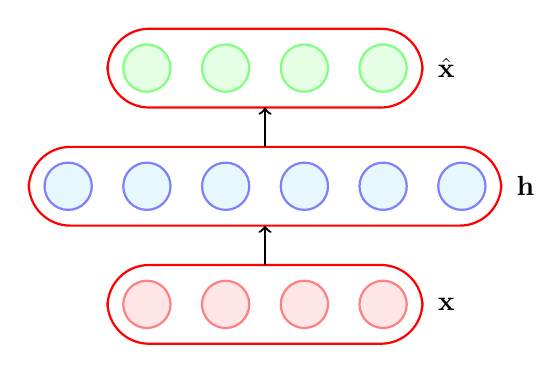
\begin{tikzpicture}

\node [input_neuron] (neuron01) at (8.5,4.5) {};
\node [input_neuron] (neuron02) at (9.5,4.5){};
\node [input_neuron] (neuron03) at (10.5,4.5) {};
\node [input_neuron] (neuron04) at (11.5,4.5) {};
\node [hidden_neuron] (neuron51) at (7.5,6) {} ;
\node [hidden_neuron] (neuron52) at (8.5,6)  {};
\node [hidden_neuron] (neuron53) at (9.5,6)  {};
\node [hidden_neuron] (neuron54) at (10.5,6)  {};
\node [hidden_neuron] (neuron55) at (11.5,6)  {};
\node [hidden_neuron] (neuron56) at (12.5,6)  {};

\node [output_neuron] (neuron11) at (8.5,7.5)  {};
\node [output_neuron] (neuron12) at (9.5,7.5)  {};
\node [output_neuron] (neuron13) at (10.5,7.5)  {};
\node [output_neuron] (neuron14) at (11.5,7.5)  {};


\node[text width=0.01cm] at (12.2,4.5) {$\textbf{x}$};
\node[text width=0.01cm] at (13.2,6) {$\textbf{h}$};
\node[text width=0.01cm] at (12.2,7.5) {$\hat{\textbf{x}}$};

\draw[red!100,thick,solid,rounded corners=15pt] (8,4) rectangle (12,5);
\draw[red!100,thick,solid,rounded corners=15pt] (7,5.5) rectangle (13,6.5);
\draw[red!100,thick,solid,rounded corners=15pt] (8,7) rectangle (12,8);


\draw[thick,->] (10,5) -- (10,5.5);

\draw[thick,->] (10,6.5) -- (10,7);

\end{tikzpicture}
\end{center}
        \tikzstyle{input_neuron}=[circle,draw=red!50,fill=red!10,thick,minimum size=6mm]
\tikzstyle{hidden_neuron}=[circle,draw=blue!50,fill=cyan!10,thick,minimum size=6mm]
\tikzstyle{output_neuron}=[circle,draw=green!50,fill=green!10,thick,minimum size=6mm]
\tikzstyle{cpy_neuron}=[circle,draw=red!50,fill=red!50,thick,minimum size=6mm]
\tikzstyle{input}=[circle,draw=black!50,fill=black!20,thick,minimum size=6mm]

\begin{center}
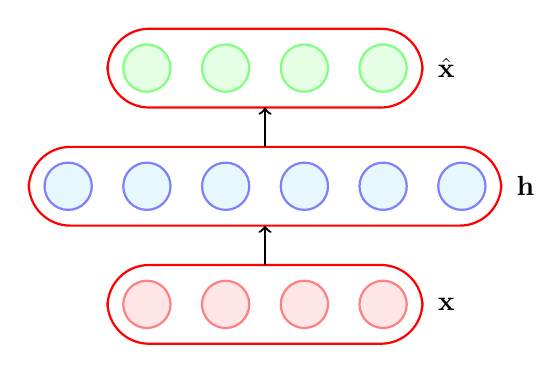
\begin{tikzpicture}

\node [input_neuron] (neuron01) at (8.5,4.5) {};
\node [input_neuron] (neuron02) at (9.5,4.5){};
\node [input_neuron] (neuron03) at (10.5,4.5) {};
\node [input_neuron] (neuron04) at (11.5,4.5) {};
\node [hidden_neuron] (neuron51) at (7.5,6) {} ;
\node [hidden_neuron] (neuron52) at (8.5,6)  {};
\node [hidden_neuron] (neuron53) at (9.5,6)  {};
\node [hidden_neuron] (neuron54) at (10.5,6)  {};
\node [hidden_neuron] (neuron55) at (11.5,6)  {};
\node [hidden_neuron] (neuron56) at (12.5,6)  {};

\node [output_neuron] (neuron11) at (8.5,7.5)  {};
\node [output_neuron] (neuron12) at (9.5,7.5)  {};
\node [output_neuron] (neuron13) at (10.5,7.5)  {};
\node [output_neuron] (neuron14) at (11.5,7.5)  {};


\node[text width=0.01cm] at (12.2,4.5) {$\textbf{x}$};
\node[text width=0.01cm] at (13.2,6) {$\textbf{h}$};
\node[text width=0.01cm] at (12.2,7.5) {$\hat{\textbf{x}}$};

\draw[red!100,thick,solid,rounded corners=15pt] (8,4) rectangle (12,5);
\draw[red!100,thick,solid,rounded corners=15pt] (7,5.5) rectangle (13,6.5);
\draw[red!100,thick,solid,rounded corners=15pt] (8,7) rectangle (12,8);


\draw[thick,->] (10,5) -- (10,5.5);

\draw[thick,->] (10,6.5) -- (10,7);

\end{tikzpicture}
\end{center}
        % The average value of the activation of a neuron $l$ is given by
        % \[ 
        %     \hat{\rho_l} = \frac{1}{m}\sum_{i=1}^m h(\textbf{x}_i)_l
        % \]
    \end{overlayarea}

    \column{0.6\textwidth}
    \begin{overlayarea}{\textwidth}{\textheight}
        \begin{itemize}\justifying
            \item<2-> A hidden neuron with sigmoid activation will have values between 0 and 1
            \item<3->We say that the neuron is activated when its output is close to 1  and not activated when its output is close to 0.  
            \item<4-> A sparse autoencoder tries to ensure the neuron is inactive most of the times.
        \end{itemize}
    \end{overlayarea}
  \end{columns}
\end{frame}

\begin{frame}
  \begin{columns}
    \column{0.4\textwidth}
    \begin{overlayarea}{\textwidth}{\textheight}
        \vspace{-0.2cm}
        % \tikzstyle{input_neuron}=[circle,draw=red!50,fill=red!10,thick,minimum size=6mm]
\tikzstyle{hidden_neuron}=[circle,draw=blue!50,fill=cyan!10,thick,minimum size=6mm]
\tikzstyle{output_neuron}=[circle,draw=green!50,fill=green!10,thick,minimum size=6mm]
\tikzstyle{cpy_neuron}=[circle,draw=red!50,fill=red!50,thick,minimum size=6mm]
\tikzstyle{input}=[circle,draw=black!50,fill=black!20,thick,minimum size=6mm]

\begin{center}
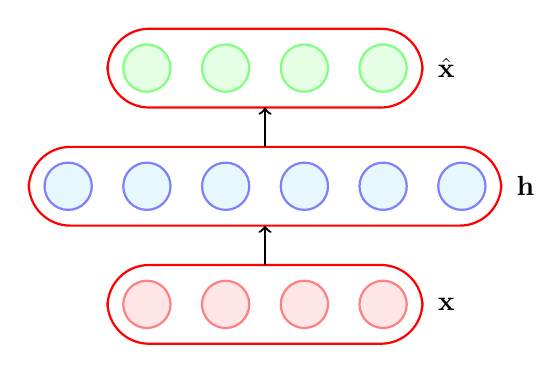
\begin{tikzpicture}

\node [input_neuron] (neuron01) at (8.5,4.5) {};
\node [input_neuron] (neuron02) at (9.5,4.5){};
\node [input_neuron] (neuron03) at (10.5,4.5) {};
\node [input_neuron] (neuron04) at (11.5,4.5) {};
\node [hidden_neuron] (neuron51) at (7.5,6) {} ;
\node [hidden_neuron] (neuron52) at (8.5,6)  {};
\node [hidden_neuron] (neuron53) at (9.5,6)  {};
\node [hidden_neuron] (neuron54) at (10.5,6)  {};
\node [hidden_neuron] (neuron55) at (11.5,6)  {};
\node [hidden_neuron] (neuron56) at (12.5,6)  {};

\node [output_neuron] (neuron11) at (8.5,7.5)  {};
\node [output_neuron] (neuron12) at (9.5,7.5)  {};
\node [output_neuron] (neuron13) at (10.5,7.5)  {};
\node [output_neuron] (neuron14) at (11.5,7.5)  {};


\node[text width=0.01cm] at (12.2,4.5) {$\textbf{x}$};
\node[text width=0.01cm] at (13.2,6) {$\textbf{h}$};
\node[text width=0.01cm] at (12.2,7.5) {$\hat{\textbf{x}}$};

\draw[red!100,thick,solid,rounded corners=15pt] (8,4) rectangle (12,5);
\draw[red!100,thick,solid,rounded corners=15pt] (7,5.5) rectangle (13,6.5);
\draw[red!100,thick,solid,rounded corners=15pt] (8,7) rectangle (12,8);


\draw[thick,->] (10,5) -- (10,5.5);

\draw[thick,->] (10,6.5) -- (10,7);

\end{tikzpicture}
\end{center}
        \tikzstyle{input_neuron}=[circle,draw=red!50,fill=red!10,thick,minimum size=6mm]
\tikzstyle{hidden_neuron}=[circle,draw=blue!50,fill=cyan!10,thick,minimum size=6mm]
\tikzstyle{output_neuron}=[circle,draw=green!50,fill=green!10,thick,minimum size=6mm]
\tikzstyle{cpy_neuron}=[circle,draw=red!50,fill=red!50,thick,minimum size=6mm]
\tikzstyle{input}=[circle,draw=black!50,fill=black!20,thick,minimum size=6mm]

\begin{center}
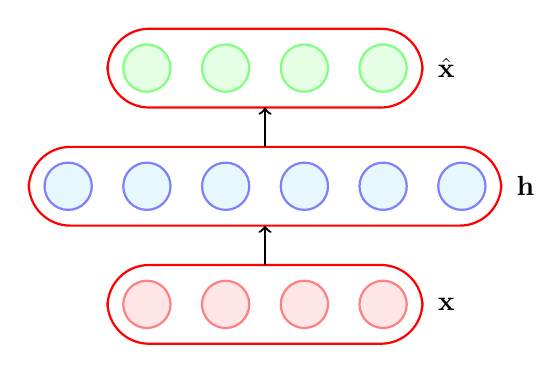
\begin{tikzpicture}

\node [input_neuron] (neuron01) at (8.5,4.5) {};
\node [input_neuron] (neuron02) at (9.5,4.5){};
\node [input_neuron] (neuron03) at (10.5,4.5) {};
\node [input_neuron] (neuron04) at (11.5,4.5) {};
\node [hidden_neuron] (neuron51) at (7.5,6) {} ;
\node [hidden_neuron] (neuron52) at (8.5,6)  {};
\node [hidden_neuron] (neuron53) at (9.5,6)  {};
\node [hidden_neuron] (neuron54) at (10.5,6)  {};
\node [hidden_neuron] (neuron55) at (11.5,6)  {};
\node [hidden_neuron] (neuron56) at (12.5,6)  {};

\node [output_neuron] (neuron11) at (8.5,7.5)  {};
\node [output_neuron] (neuron12) at (9.5,7.5)  {};
\node [output_neuron] (neuron13) at (10.5,7.5)  {};
\node [output_neuron] (neuron14) at (11.5,7.5)  {};


\node[text width=0.01cm] at (12.2,4.5) {$\textbf{x}$};
\node[text width=0.01cm] at (13.2,6) {$\textbf{h}$};
\node[text width=0.01cm] at (12.2,7.5) {$\hat{\textbf{x}}$};

\draw[red!100,thick,solid,rounded corners=15pt] (8,4) rectangle (12,5);
\draw[red!100,thick,solid,rounded corners=15pt] (7,5.5) rectangle (13,6.5);
\draw[red!100,thick,solid,rounded corners=15pt] (8,7) rectangle (12,8);


\draw[thick,->] (10,5) -- (10,5.5);

\draw[thick,->] (10,6.5) -- (10,7);

\end{tikzpicture}
\end{center}
        The average value of the activation of a neuron $l$ is given by
        \[ 
            \hat{\rho}_l = \frac{1}{m}\sum_{i=1}^m h(\textbf{x}_i)_l
        \]
        %\end{onlyenv}
    \end{overlayarea}

    \column{0.6\textwidth}
    \begin{overlayarea}{\textwidth}{\textheight}
        \begin{itemize}\justifying
            \item<1-> If the neuron $l$ is sparse (i.e. mostly inactive) then $\hat{\rho}_{l} \rightarrow 0$
            \item<2->A sparse autoencoder uses  a sparsity parameter $\rho$ (typically very close to 0, say, 0.005) and tries to enforce the constraint $\hat{\rho}_{l} = \rho$
            \item<3-> One way of ensuring this is to add the following term to the objective function\\
                \[
                    \Omega(\theta) = 
                        \sum_{l=1}^k \rho \log \frac{\rho}{\hat{\rho}_l} + 
                        (1-\rho) \log \frac{1-\rho}{1-\hat{\rho}_{l}}
                \]
            \item<4->When will this term reach its minimum value and what is the minimum value? Let us plot it and check.
        \end{itemize}
    \end{overlayarea}
  \end{columns}
\end{frame}

\begin{frame}
	
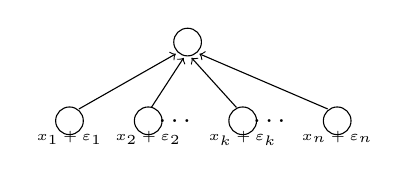
\begin{tikzpicture}
	\begin{scope}[every node/.style={sloped,allow upside down}]
		\draw (1.5,3) circle (0.5em);
		\draw (0,2) circle (0.5em)
		node[below=0.15] {\tiny $x_1 + \varepsilon_1$};
		\draw (1,2) circle (0.5em)
		node[below=0.15] {\tiny $x_2 + \varepsilon_2$}
		node[right=0.19] {\dots};
		\draw (2.2,2) circle (0.5em)
		node[below=0.15] {\tiny $x_k + \varepsilon_k$}
		node[right=0.19] {\dots};
		\draw (3.4,2) circle (0.5em) node[below=0.15] {\tiny $x_n + \varepsilon_n$};
		\draw[->] (0.12,2.15) -- (1.35,2.85);
		\draw[->] (1.04,2.17) -- (1.45,2.8);
		\draw[->] (2.12,2.17) -- (1.55,2.8);
		\draw[->] (3.28,2.15) -- (1.65,2.85);
	\end{scope}
\end{tikzpicture}

    \begin{itemize}\justifying
        \item<2-> The function will reach its minimum value(s) when $\hat{\rho}_{l} = \rho$.
    
\end{itemize}
%}
%\end{overlayarea}
%\end{columns}
\end{frame}

\begin{frame}
  \begin{columns}
    \column{0.55\textwidth}
    \begin{overlayarea}{\textwidth}{\textheight}
        %\begin{itemize}
            \footnotesize{
            \onslide<5-> 
            \[ 
                \Omega(\theta) = \sum_{l=1}^k \rho log \frac{\rho}{\hat{\rho}_{l}} + (1-\rho)log\frac{1-\rho}{1-\hat{\rho}_{l}}
            \]
            \onslide<6-> Can be re-written as
            \[
                \Omega(\theta) = \sum_{l=1}^k \rho log \rho - \rho log \hat{\rho}_{l} + (1-\rho) log (1-\rho) - (1-\rho) log (1-\hat{\rho}_{l})
            \]
            \onslide<7-> By Chain rule:
            \[
                \frac{\partial{\Omega(\theta)}}{\partial{W}} = \frac{\partial{\Omega(\theta)}}{\partial{\mathbf{\hat{\rho}}}}.\frac{\partial{\mathbf{\hat{\rho}}}}{\partial{W}}
            \]
            \onslide<8-> 
            {\[
	          	 \frac{\partial{\Omega(\theta)}}{\partial{\mathbf{\hat{\rho}}}} = \begin{bmatrix}
	          	  \frac{\partial{\Omega(\theta)}}{\partial{\hat{\rho}_1}} , \frac{\partial{\Omega(\theta)}}{\partial{\hat{\rho}_2}} ,\dots  \frac{\partial{\Omega(\theta)}}{\partial{\hat{\rho}_k}} 
	          	 \end{bmatrix}^T
	         \]}
	         \onslide<9->{          
            For each neuron $l \in 1 \dots k$ in hidden layer, we have
\vspace{-0.5cm}}
	         
	         \begin{align*}
	           \onslide<10->{\frac{\partial{\Omega(\theta)}}{\partial{\hat{\rho}_l}} &= -\frac{\rho}{\hat{\rho}_l} + \frac{(1-\rho)}{1-\hat{\rho}_l}\\}
	           \onslide<11->{\text{and}\qquad
                 	\frac{\partial{\hat{\rho}_{l}}}{\partial{W}} &= \textbf{x}_{i}(g'(W^{T}\textbf{x}_{i} + \mathbf{b}))^{T} \text{(see next slide)}}
	         \end{align*}
              
            
            
            }
        %\end{itemize}
    \end{overlayarea}

    \column{0.45\textwidth}
    \small
    \begin{overlayarea}{\textwidth}{\textheight}
        \begin{itemize}\justifying
            \onslide<1-> \item Now,
                \[
                    \hat{\mathscr{L}}(\theta) = \mathscr{L}(\theta) + \Omega(\theta)
                \]
            \vspace{-0.5cm}
            \onslide<2-> \item $\mathscr{L}(\theta)$ is the squared error loss or cross entropy loss and $\Omega(\theta)$ is the      sparsity    constraint.
            \onslide<3-> \item We already know how to calculate $\frac{\partial\mathscr{L}(\theta)}{\partial W}$
            \onslide<4-> \item Let us see how to calculate $\frac{\partial{\Omega(\theta)}}{\partial{W}}$.
            \onslide<12->\item Finally,
            \[
                \frac{\partial{\hat{\mathscr{L}}(\theta)}}{\partial{W}} = \frac{\partial{\mathscr{L}(\theta)}}{\partial{W}} + \frac{\partial{\Omega(\theta)}}{\partial{W}}
            \]
            (and we know how to calculate both terms on R.H.S)
        \end{itemize}
    \end{overlayarea}
  \end{columns}
\end{frame}


\begin{frame}
\small
    \begin{overlayarea}{\textwidth}{\textheight}
    \vspace{0.025cm}
    \underline{\textbf{Derivation}}
\[
    \frac{\partial \hat{\rho}}{\partial W} = \begin{bmatrix}
    \frac{\partial \hat{\rho}_1}{\partial W} & \frac{\partial \hat{\rho}_2}{\partial W} \dots \frac{\partial \hat{\rho}_k}{\partial W}
    \end{bmatrix}
\]
    For each element in the above equation we can calculate $\frac{\partial \hat{\rho}_l}{\partial W}$ (which is the partial derivative of a scalar w.r.t. a matrix = matrix).
    For a single element of a matrix $W_{jl}$:-
    \begin{align*}
	\frac{\partial \hat{\rho}_l}{\partial W_{jl}} &= \frac{\partial \Big[ \frac{1}{m} \sum_{i=1}^{m} g \big( W_{:,l}^{T}\mathbf{x_i}+b_l\big) \Big] }{\partial W_{jl}}\\
	&= \frac{1}{m} \sum_{i=1}^{m}\frac{\partial \Big[ g \big( W_{:,l}^{T}\mathbf{x_i}+b_l\big) \Big] }{\partial W_{jl}}\\
	&= \frac{1}{m} \sum_{i=1}^{m} g' \big( W_{:,l}^{T}\mathbf{x_i}+b_l\big) x_{ij}
    \end{align*}
    \vspace{-0.1cm}
    So in matrix notation we can write it as :
    \begin{align*}
    \frac{\partial{\hat{\rho}_{l}}}{\partial{W}} = \textbf{x}_{i}(g'(W^{T}\textbf{x}_{i} + \mathbf{b}))^{T} 
    \end{align*}
	\end{overlayarea}
\end{frame}

% Slide 44 Module 5 ends here

